\section{Evaluation}
\label{thesy:evaluation}

We implemented \TheSy in Rust, using the e-graph manipulation library \emph{egg}~\cite{egg}.
\TheSy accepts definitions in SMTLIB-2.6 format~\cite{TR2017:Barrett},
based on the UF theory (uninterpreted functions),
limited to universal quantifications.
Type declarations occurring in the input are collected and comprise $\Vocab$;
universal equalities form $\Eqs$ and are translated into rewrite rules (either uni- or bidirectional, as explained in \autoref{prelim:term-rewriting}).
Then SyGuE is performed on $\Vocab$, generating candidate conjectures using SOE.
SyGuE uses \emph{egg} for equivalence reduction, and SOE uses it for comparing symbolic values. Conjectures are then dismissed using \TheSy's induction-based prover.
This is done in an iterative deepening loop.

\begin{paragraph}{Case split\quad}
Both SOE and the prover use a case splitting mechanism; This mechanism detects when rewriting cannot match due to an opaque value (an uninterpreted symbol), and applies case splitting according to the constructors of relevant ADTs.
However, doing so for every rule is too costly and, in most cases, redundant --- \TheSy generates a variety of terms, so if one term is blocked due to an uninterpreted symbol, another one exists with a symbolic example instead.
A situation where this is \emph{not} the case is when \emph{multiple} uninterpreted symbols block the rewrite (recall that \TheSy only substitutes one placeholder per term with symbolic examples). 
To illustrate, consider the case in \autoref{overview:induction-example} where both the list $\clrterm x::xs$ and $\clrterm p\,x$ are used in match expressions, therefore a case split is needed by ${\clrterm p\,x} \in \{\ttrue,\tfalse\}$.
Therefore, \TheSy only performs case splitting for rewrite rules that require multiple match patterns but only one is blocked.

The splitting mechanism itself, operates by copying the e-graph and applying the term rewriting logic separately for each case. 
Each copy then yields a partition of the existing equivalence classes. 
These partitions are intersected between all cases, and each of the resulting intersections lead to merging of equivalence classes in the original e-graph.
It is worth noting that \TheSy never needs to backtrack a case split it has elected to apply.
As a consequence, execution time is not exponential in the total number of case splits performed, only in the nesting level of such splits (which is bounded by 2 in our experiments). 
\end{paragraph}

\begin{comment} 
The better known but opposed approach is the common SMT solver approach (Barrett et al., Gil et al.). In the SMT approach, the solver attempts to search for a legal valuation, and assumptions are made freely. This leads to a cheap splitting mechanism, but with an expensive backtracking algorithm. We evaluated our case splitting mechanism by applying TheSy to Clam’s (Claessen et al.) theory-proving dataset with three configurations: no case splitting - default implementation; half case splitting – splitting was applied only during proof search; and full  case splitting – splitting was applied for both exploration and proof search. Each test case was limited to 15 minutes and 16 GB RAM, and the results are shown in Table 1. Additionally, we report the number of lemmas found in the full configuration compared to the half configuration and the number of proofs filtered in each configuration. An interesting point is that the no and full configurations had 53 and 54 goals proved, respectively. This difference is due to full configuration time-outing during case splitting in which regular exploration is sufficient. Using the half configuration, TheSy proved 61 goals which mostly overlap with the previous configurations as it is less prune to time-outs. In total, TheSy proved 63 out of the 85 goals. Memory and time limits lead to most of the full case splitting failures. Case splitting during exploration led to additional conjectures and lemmas; many conjectures were filtered only after proving their correctness, a phenomenon which impaired the conjecture generation/screening process. This happened because TheSy’s e-graph size is limited for memory concerns, resulting in an unsound screening process .
\end{comment}

We compare \TheSy to the most recent and closely related theory exploration system, Hipster~\cite{hipster}---which is
based on random testing (backed by QuickSpec~\cite{JFP2017:Smallbonequickspec2}) with proof automations from and frontend in Isabelle/HOL~\cite{Book2002:Nipkow}.
Hipster represents the culmination of several works on existing theory exploration (see~\autoref{thesy:related}).
Both systems generate a set of proved lemmas as output, each such set encompassing a conceptual volume of knowledge that was discovered automatically.
We note that the same knowledge can be represented in various ways, so directly comparing the sets of lemmas is going to be meaningless.

\subsection{Evaluating Theory Exploration Quality}

We define a comparison method for two theory exploration systems $A$ and $B$ starting from a common initial theory (defined as a set of closed formulas) $\mathcal{T}$.
As a metric for the quality and efficacy of results obtained from theory exploration, and, therefore, their perceived usefulness, we use the notion of \emph{knowledge} (inspired by ``knowledge base'' in Theorema~\cite{Journal2002:Buchberger}).
A theory $\mathcal{T}$ in a given logical proof system induces a collection of attainable knowledge, $\mathcal{K}_\mathcal{T} = \left\{\varphi ~\rule[-2.5pt]{0.5pt}{9.5pt}~ \mathcal{T}\vdash\varphi\right\}$,
that is, characterized by the set of (true) statements that can be proven based on $\mathcal{T}$.
In practice, a ``pure'' notion of knowledge based on provability is impractical, because most interesting logics are undecidable,
and automated proving techniques cannot feasibly find proofs for all true statements.
We, therefore, parameterize knowledge relative to a \emph{prover} --- a procedure that always terminates and can prove a subset of true statements.
Termination can be achieved by restricting the space of proofs by either size or resource bounds.
We say that $\mathcal{T}
\vdash^{^{\hspace{-.4em}S\hspace{-.2em}}} \varphi$ when a prover, $S$, is able to verify the validity of $\varphi$ in a theory $\mathcal{T}$.
A more realistic characterization of knowledge would then be
$\mathcal{K}_\mathcal{T}^S = \big\{\varphi ~{\rule[-3pt]{0.5pt}{11.5pt}}~
\mathcal{T}\prvbySinline\varphi\big\}$.
Assuming that the prover $S$ is fixed, a theory $\mathcal{T}'$ is said to \emph{increase knowledge} over $\mathcal{T}$ when
$\mathcal{K}_{\mathcal{T}'}^S \supset \mathcal{K}_{\mathcal{T}}^S$.
%\end{paragraph}

We utilize the notion of $\mathcal{K}_\mathcal{T}^S$ described above to test the knowledge gained by $A$ against that of $B$, and vice versa.
We take the set of lemmas $\mathcal{T}_A$ generated by $A$ and check whether it is subsumed by $\mathcal{T}_B$, generated by $B$, by checking whether $\mathcal{T}_A\subseteq \mathcal{K}_{\mathcal{T}\cup\mathcal{T}_B}^S$;
we then carry out the same comparison with the roles of $A$ and $B$ reversed.
A working assumption is that both $A$ and $B$ include some mechanism for screening redundant conjectures.
That is, a component that receives the current set of known lemmas $T_i$ and a conjecture $\varphi$ and decides whether the conjecture is redundant.
It is important to choose $S$ such that whenever $A$ (or $B$) discards $\varphi$, due to redundancy, it holds that $\varphi \in \mathcal{K}_{T_i}^S$.

\begin{figure}[t]
    \newcommand\tthesy{\textrm{T}}
\newcommand\thipster{\textrm{H}}

\newcommand\fwith{w\hspace{-1pt}/\hspace{-1pt}\xspace}
\newcommand\fwithout{w\hspace{-1pt}/\hspace{-1pt}o\xspace}


\begin{tikzpicture}
\coordinate (O) at (0,0);
\begin{axis}[
    title={\TheSy {\smaller~(\fwithout case split)} \vs Hipster},
    at=(O),
    %enlargelimits=false,
    draw={black!30!white},
    width=5.5cm, height=5.5cm,
    grid=both,
    xmin=0, xmax=1,
    ymin=0, ymax=1,
    ticklabel style={font=\tiny},
    x label style={at={(axis description cs:0.5,-0.07)},anchor=north},
    y label style={at={(axis description cs:-0.1,.5)},rotate=-90,anchor=east},
    xlabel={$\mathcal{T}_{\thipster} \cmptheories
             \mathcal{T}_{\tthesy}$},
    ylabel={$\mathcal{T}_{\tthesy} \cmptheories
             \mathcal{T}_{\thipster}$}
]
\addplot[  
    only marks,
    scatter,
    scatter src=y-x,
    point meta min=-.6, point meta max=1,
    mark size=1.25pt]
table[x=t<h,y=h<t]{thesy/img/scatter-plot-no-cs.dat.txt};
\end{axis}
%
\draw[color=olive!60!white] (O) -- +(4cm, 4cm);

% ----------------------------------

\coordinate (O) at (6.3cm,0);
\begin{axis}[
    title={\TheSy {\smaller~(\fwith case split)} \vs Hipster},
    at=(O),
    %enlargelimits=false,
    draw={black!30!white},
    width=5.5cm, height=5.5cm,
    grid=both,
    xmin=0, xmax=1,
    ymin=0, ymax=1,
    ticklabel style={font=\tiny},
    x label style={at={(axis description cs:0.5,-0.07)},anchor=north},
    y label style={at={(axis description cs:-0.1,.5)},rotate=-90,anchor=east},
    xlabel={$\mathcal{T}_{\thipster} \cmptheories
             \mathcal{T}_{\tthesy}$},
    ylabel={$\mathcal{T}_{\tthesy} \cmptheories
             \mathcal{T}_{\thipster}$}
]
\addplot[  
    only marks,
    scatter,
    scatter src=y-x,
    point meta min=-.5, point meta max=1,
    mark size=1.25pt]
table[x=t<h,y=h<t]{thesy/img/scatter-plot-with-cs.dat.txt};
\end{axis}
%
\draw[color=olive!60!white] (O) -- +(4cm, 4cm);
%
\end{tikzpicture}
%
\vspace{-2em}  % why does it make this space? 
    \caption{A scatter plot showing the ratio of lemmas in theories discovered by each tool that were subsumed by the theory discovered by its counterpart ($\tthesy$ = \TheSy, $\thipster$ = Hipster). Each point represents a single test case.
    The vertical axis shows how many of the lemmas discovered by Hipster were subsumed by those discovered by \TheSy, and the horizontal axis shows the converse.}
    \label{results:ratio_chart}
\end{figure}

Incorporating the solver into the comparison makes the evaluation resistant to large amounts of trivial lemmas, as they will be discarded by A or B.
It is still possible for some lemmas to be ``better'' than others, so knowledge is not uniformly distributed; this is hard to quantify, though.
A few possible measures of usefulness come to mind, such as lemma utilization in a task (such as proof search), proof complexity, or matching to a given context, but given just the exploration task, there is not sufficient information to apply them.
A first approximation is to consider the discovered lemmas themselves, \ie,
$\mathcal{T}_A \cup \mathcal{T}_B$, as representing proof objectives.
In doing so, we pit $A$ and $B$ in direct contest with one another.
We choose this avenue because it is straightforward to apply, admitting that it may be inaccurate in some cases.

To evaluate our approach and its implementation, we run both \TheSy and Hipster
on functional definitions collected from the TIP 2015 benchmark suite~\cite{CICM2015:Claessen}, specifically the IsaPlanner~\cite{ITP2010:Johansson} benchmarks (85 benchmarks in total), for compatibility between the two systems.
TIP benchmarks also contain goal propositions, but for the purpose of evaluating the exploration technique, these are redacted.
%We compare the results of running \TheSy against those exhibited by Hipster,
%a theory exploration based on random testing (backed by QuickSpec~\cite{JFP2017:Smallbonequickspec2}) with a frontend for Isabelle/HOL~\cite{Book2002:Nipkow}.
%To compare the outputs, we use the notion of knowledge described in \autoref{technical}:
%Given two theories $\mathcal{T}_1, \mathcal{T}_2$, we check every lemma $\varphi\in\mathcal{T}_1$ against $\mathcal{T}_2$, and vice versa;
This experiment uses the simple rewrite-driven congruence-closure decision procedure with a case split mechanism in the role of the solver, $S$, occurring in the definition of knowledge $\mathcal{K}$.
Hipster uses Isabelle/HOL's simplifier as a conjecture redundancy filtering mechanism, which is in itself a simple rewrite-driven decision procedure, therefore $S$ provides a suitable comparison.
We compute the portion of lemmas found by Hipster that were provable (by $S$) from \TheSy's results and vice versa.
In other words, we check the ratio given by $| \mathcal{T}_A \cap \mathcal{K}_{\mathcal{T}\cup\mathcal{T}_B}^S | \,/\, | \mathcal{T}_A |$, which we denote $\mathcal{T}_B\cmptheories\mathcal{T}_A$, in both directions.
\autoref{results:ratio_chart} displays the ratios, where each point represents a single test case.
Points above the diagonal line represent test cases where \TheSy's ratio was higher and for points under the line Hipster's ratio was higher.
We conduct this experiment twice: Once with the case-splitting mechanism of \TheSy turned off for its exploration, and once with it turned on. (Hipster does not have such a switch as it always generates concrete values.)
The reason for this is that case splitting increases the running time significantly (as we show next), so we want to evaluate its contribution to the discovery of lemmas.
Comparing the two charts, while \TheSy performs reasonably well compared to Hipster without case splitting (in 48 out of the 85 \TheSy's ratio was better and equal in 12), enabling it leads to a clear advantage (in 65 out of the 85 \TheSy's ratio was better and equal in 6).


\begin{figure}[t]
\centering
%\renewcommand\arraystretch{1.3}
\setlength{\tabcolsep}{4pt}
\begin{tabular}{|l@{~~~}|r|r|r|r|r|r|r|r|r|r|}
\cline{2-11}
\multicolumn{1}{l|}{}
                              & 10\%         & 20\% & 30\% & 40\% & 50\% & 60\% & 70\% & 80\% & 90\% & 100\% \\ \hline
\TheSy   & \textless{}1 & 2    & 6    & 12   & 46   & 113  & 792  & 8.3K & 39K  & 68K   \\ \hline
Hipster  & 380          & 1.3K & 3K   & 5.2K & 7.8K & 11K  & 16K  & 23K  & 34K  & 47K   \\ \hline
\end{tabular}
\vspace{3pt}
%\newcommand\slightlysmaller{\fontsize{7pt}{7pt}\selectfont}

\begin{tikzpicture}
  \begin{axis}[
  		width=9cm,
        height=6cm,
        xmin=-2,
        xmax=89,
        xtick distance=15,
        extra x ticks={85},
        ymode=log,
        ytick distance=10^1,
        ymajorgrids=true,
        xlabel={benchmarks solved},
        ylabel={accumulated time\, 
           (\textit{s}\hspace{.75pt})},
           mark size=.5pt,
        legend style={
          anchor=north west,
          font={\fontsize{7.5pt}{7.5pt}\selectfont}
        },
        legend image post style={mark size=2pt, scale=0.8},
        legend cell align={left}]
        
    \addplot[smooth,mark=*,mark size=.6pt,mark options={fill=white},green!50!gray] plot 
      table[y=hipster] {thesy/img/cactus-plot-with-cs.dat.txt};
    \addlegendentry{Hipster}

    \addplot[smooth,mark=*,orange!50!red] plot 
       table[y=thesy] {thesy/img/cactus-plot-with-cs.dat.txt};
    \addlegendentry{TheSy\,%
    {\smaller(w\hspace{-1pt}/\hspace{-1pt} case split)}}

    \addplot[smooth,mark=x,mark size=1.1pt,purple] plot 
       table[y=thesy] {thesy/img/cactus-plot-no-cs.dat.txt};
    \addlegendentry{TheSy\,%
    {\smaller(w\hspace{-1pt}/\hspace{-1pt}o case split)}}

  \end{axis}
\end{tikzpicture}

\vspace{-2em}
\caption{Time to fully explore the 85 IsaPlanner benchmarks.
A full exploration is considered one where either all terms up to the depth bound have been enumerated or a timeout of 1hr has been reached.
The $y$ axis shows the amount of time needed to complete the first $x$ benchmarks, when they are sorted from shortest- to longest-running.
(Time scale is logarithmic; lower is better.)}
\label{results:time-perc-table}
\end{figure}

\subsubsection{Performance}

To compare runtime efficiency, we consider the time it took to fully explore the IsaPlanner test suite.
We consider an exploration ``full'' when it has finished enumerating all the terms, and associated candidate conjectures, up to the depth bound ($k=2$)\footnote{Our experience shows that choosing larger $k$s greatly affects the run-time, but does not lead to many useful lemmas.} with \TheSy or size bound with Hipster ($s=7$), and check them; or when a timeout of one hour is reached, whichever is sooner.
We then sort the benchmarks from shortest- to longest-running for each of the tools, and report the accumulated time to explore the first $i$ benchmarks ($i=1..85$).
The results are shown in the graph in \autoref{results:time-perc-table}, for Hipster, \TheSy with case split disabled, and \TheSy with case split enabled.
In both configurations, \TheSy is very fast for the lower percentiles, but begins to slow down, due to case splitting, towards the end of the line.
To illustrate, in the 25th percentile \TheSy was {\raise.17ex\hbox{$\scriptstyle\sim$}}380 times faster (0.48s \vs 182.47s); in the 50th percentile, {\raise.17ex\hbox{$\scriptstyle\sim$}}57 times faster (5.28s \vs 305.37s); and in the 75th percentile, {\raise.17ex\hbox{$\scriptstyle\sim$}}6 times faster (141.24 to 883.8).
Overall \TheSy took 51.6K seconds and Hipster 47.1K, meaning Hipster was {\raise.17ex\hbox{$\scriptstyle\sim$}}1.1 times faster.
It is evident from the chart that case splitting is largely responsible for the longer execution times. Without case splitting, \TheSy is much faster, and completes all 85 benchmarks in less time than it takes Hipster.
Of course, in that mode of operation, \TheSy finds fewer lemmas (as shown in \autoref{results:ratio_chart}), but is still superior to Hipster.
Future work needs to focus on improving the case-splitting mechanism, similar to their treatment in SAT and SMT, allowing \TheSy to deal with such theories more efficiently.

\subsection{Efficacy to automated proving}

While the mission statement of \TheSy is solely to provide lemmas based on core theories,
we wish to claim that such discovered theories are beneficial toward proving theorems in general, based on the same core theory.
We used a collection of benchmarks for induction proofs used by CVC4~\cite{cvc4induction}, and conducted the following experiment: First, the proof goals are skipped and only the symbol declarations and provided axioms are used to construct an input to \TheSy.
Then, whenever a new lemma is discovered and passes through the prover, we also attempt to prove the goal---utilizing the same mechanism used for vetting conjectures.
As soon as the latter goes through, the exploration process is aborted, and all lemmas collected are discarded.
The experiments are thus independent across the individual benchmarks.

Even though this setting is unfavorable to \TheSy---because it does not take advantage of the fact that theory exploration can be done offline, then its results re-used for proofs over the same core theory---we report considerable success in solving these benchmarks.
Out of the 311 benchmarks, our theory exploration + simple-minded induction was able to prove 187 (with a 5-minute timeout, same as in the original CVC4 experiments).
For comparison, Z3 and CVC4 (without conjecture generation) were able to prove 75 and 70 of them, respectively.
This shows that the majority of instances were not solvable without the use of induction.
CVC4 with its conjecture generation enabled was able to solve 260 of them.
\autoref{results:solve-table} shows the number of successful proofs achieved for each of the four suites.
\autoref{results:solve-accum} shows the accumulated time required for the benchmarks; the vast majority of the success cases occur early on, because in some cases a rather small auxiliary lemma is all that is needed to make the proof go through.

\begin{table}[t]
\centering
\renewcommand\arraystretch{1.1}
\newcommand\cc[1]{~~#1~~}
\newcommand\ctwo[1]{\multicolumn{2}{c|}{~~#1~}}
\begin{tabular}{l|r|rrrr}
           & \cc{Total} & \cc{~~Z3} & \cc{CVC4} & \cc{CVC4+ig} & \cc{\TheSy} \\ \hline
clam       & 136   & 25 & 20~   & 108~~~        & 102    \\
hipspec    & 42    & 6  & 7~    & 33~~~         & 29    \\
isaplanner & 87    & 35 & 34~   & 79~~~         & 47    \\
leon       & 46    & 9  & 9~    & 40~~~         & 9     \\ \hline
Total      & 311   & 75 & 70~   & 260~~~        & 187  
\end{tabular}
\hspace{2pt}
\vspace{5pt}
\caption{Results of the CVC4 benchmark suite (number of successful proofs in each category).}
\label{results:solve-table}
\end{table}

\begin{figure}[t]
    \centering
    %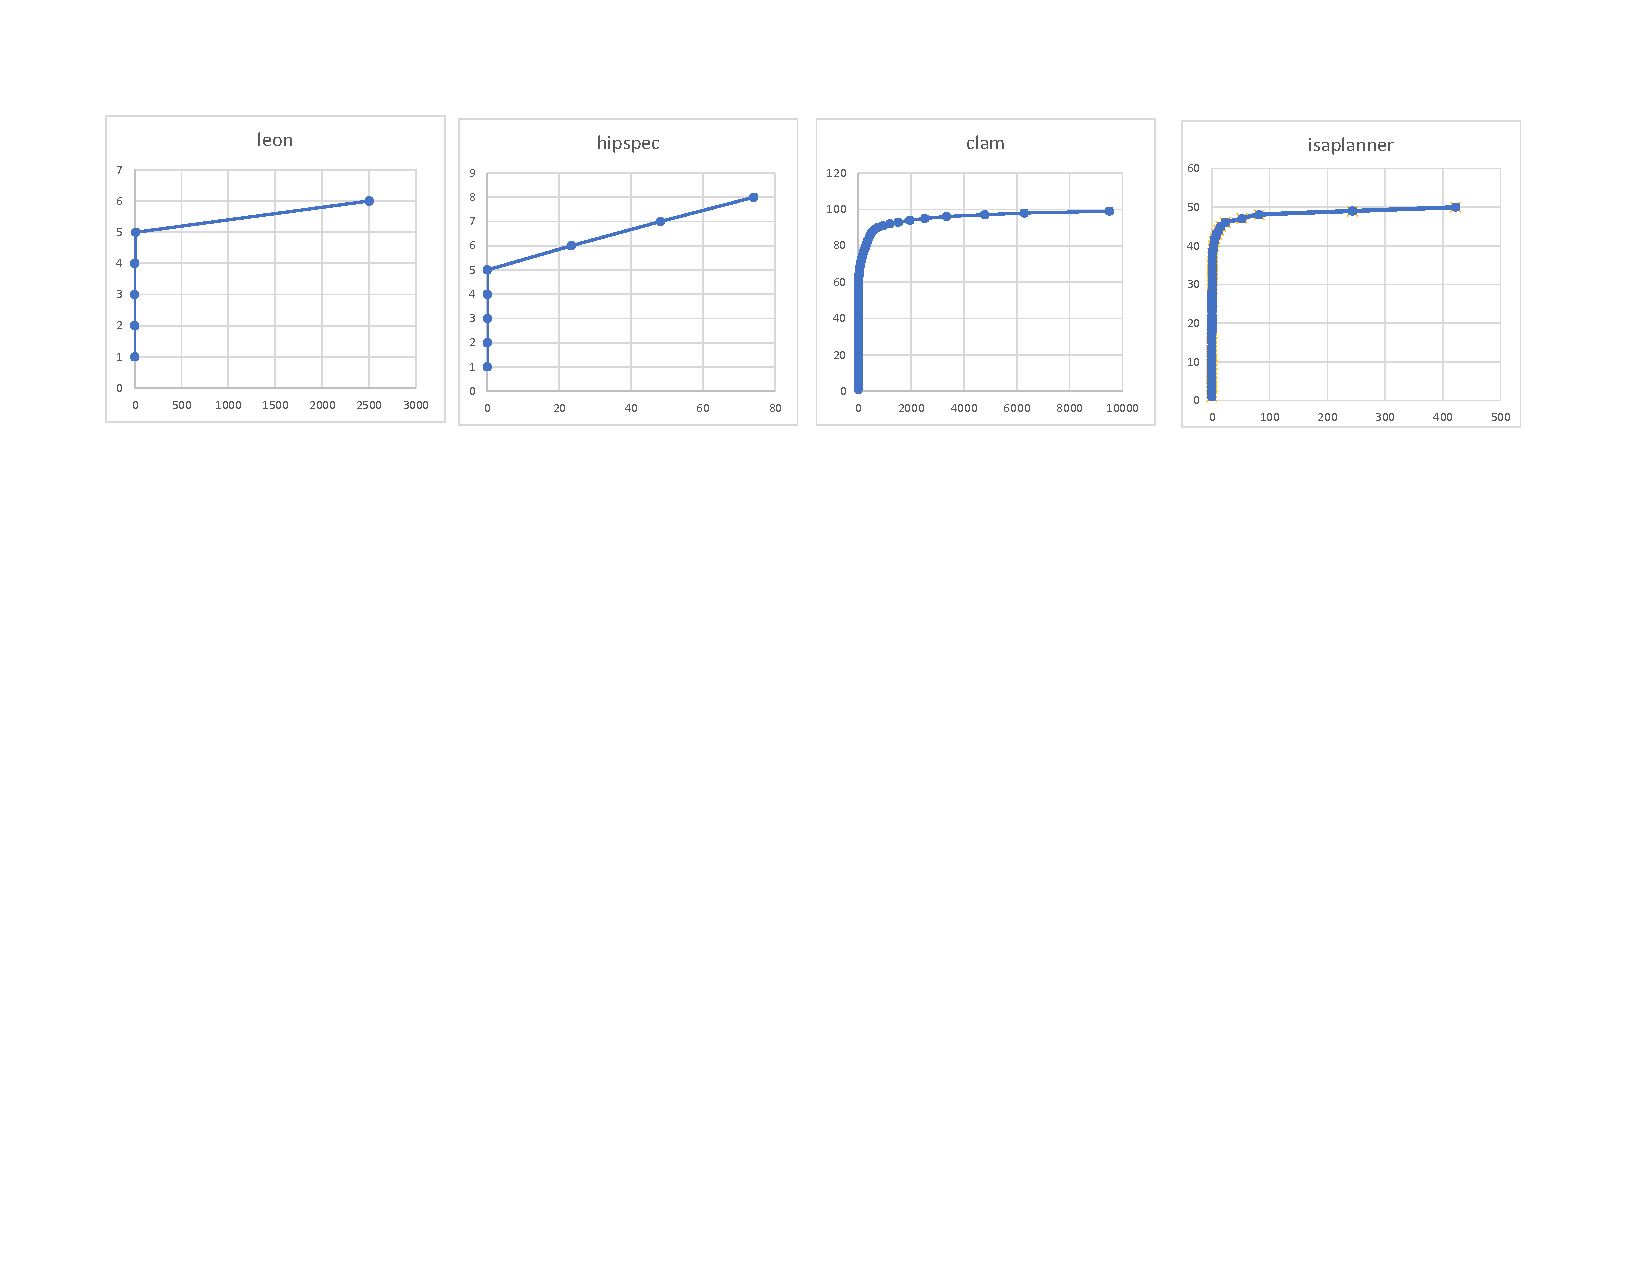
\includegraphics[width=\textwidth]{img/chart_solve_accum.pdf}
    %\newcommand\smaller{\fontsize{7pt}{7pt}\selectfont}

\begin{tikzpicture}
  \pgfplotsset{cactus/.style={
  		width=5cm,
        height=4cm,
        title style={yshift=-1pt,anchor=base},
        ytick distance=10^1,
        x tick label style={font={\smaller}},
        y tick label style={font=\tiny},
        ymajorgrids=true,
        %xlabel={benchmarks solved},
           mark size=.25pt}}

  \begin{axis}[title={clam}, cactus, ymode=log]
    \addplot[smooth,mark=*,green!50!gray] plot 
      table[y=time] {thesy/img/cvc4-benchmarks/cactus-clam.dat.txt};
  \end{axis}

  \begin{axis}[title={hipspec}, at={(5cm,0)}, cactus, ymode=log]
    \addplot[smooth,mark=*,green!50!gray] plot 
      table[y=time] {thesy/img/cvc4-benchmarks/cactus-hipspec.dat.txt};
  \end{axis}

  \begin{axis}[title={leon}, at={(0,-3.5cm)}, cactus, ymode=log]
    \addplot[smooth,mark=*,green!50!gray] plot 
      table[y=time] {thesy/img/cvc4-benchmarks/cactus-leon.dat.txt};
  \end{axis}

  \begin{axis}[title={isaplanner}, at={(5cm,-3.5cm)}, cactus, ymode=log]
    \addplot[smooth,mark=*,green!50!gray] plot 
      table[y=time] {thesy/img/cvc4-benchmarks/cactus-isaplanner.dat.txt};
  \end{axis}


\end{tikzpicture}

    \caption{Accumulated time-to-solve for each of the benchmark suites from the CVC4 collection.
    The $y$ axis shows the amount of time needed to complete the first $x$ (successful) proofs, when benchmarks are sorted from shortest- to longest-running.}
    \label{results:solve-accum}
\end{figure}